% What a KV Cache Retention Signal Must Achieve
%
% Self-contained: plain `article`, no venue style file required.
% To switch to a venue style, replace the documentclass/geometry block with
% e.g. \usepackage{neurips_2026} and delete the \geometry line.
%
% Every number that comes from an experiment is a macro or a table defined in
% tables.tex, which scripts/make_latex.py generates from results/*.json.
% Regenerate it rather than editing numbers here.
%
% Build:  pdflatex paper && bibtex paper && pdflatex paper && pdflatex paper
\documentclass[10pt]{article}
\usepackage[margin=1in]{geometry}
\usepackage[T1]{fontenc}
\usepackage[utf8]{inputenc}
\usepackage{booktabs}
\usepackage{amsmath}
\usepackage{tikz}
\usepackage{xcolor}
\usepackage{natbib}
\usepackage[hidelinks]{hyperref}
\usepackage{microtype}

\definecolor{tealaccent}{HTML}{0E7C86}
\definecolor{rustaccent}{HTML}{B0541F}

% Generated by scripts/make_latex.py from results/*.json. Do not edit.
\newcommand{\OracleSmall}{40/40}
\newcommand{\OracleLarge}{24/24}
\newcommand{\RecentSmall}{10/40}
\newcommand{\RecentLarge}{6/24}
\newcommand{\CovMidFull}{7/7}
\newcommand{\CovMidThreeQ}{1/7}
\newcommand{\ScreenSpansNeedle}{64}
\newcommand{\ScreenSpansQA}{62}
\newcommand{\RandomWholeQA}{5/62}
\newcommand{\AnswerShapeWholeQA}{15/62}
\newcommand{\AnswerShapeWholeNeedle}{0/64}
\newcommand{\ScreenBestWhole}{15/62}
\newcommand{\SurprisalNeedle}{0.105}
\newcommand{\SurprisalQA}{0.243}
\newcommand{\LookaheadNeedle}{0.181}
\newcommand{\LookaheadQA}{0.245}
\newcommand{\AnswershapeNeedle}{0.550}
\newcommand{\AnswershapeQA}{0.472}
\newcommand{\NormattentionNeedle}{0.229}
\newcommand{\NormattentionQA}{0.223}
\newcommand{\AnswerShapeRatio}{2.2}
\newcommand{\FragP}{0.0078}
\newcommand{\HorizonInside}{2/32}
\newcommand{\HorizonBeyond}{0/32}
\newcommand{\HorizonBeyondUpper}{0.11}
\newcommand{\RecentBeyond}{0/48}
\newcommand{\RecentBeyondUpper}{0.07}
\newcommand{\CrowdPred}{0.38}
\newcommand{\CrowdPredScaled}{0.30}
\newcommand{\CrowdObs}{9/24}
\newcommand{\CrowdObsCI}{[0.21, 0.57]}
\newcommand{\QACeiling}{0.79}
\newcommand{\DeadK}{0}
\newcommand{\DeadN}{340}
\newcommand{\DeadUpper}{1.1\%}
\newcommand{\DeadQA}{1/64}
\newcommand{\DeadQAUpper}{8.3\%}
\newcommand{\DeadQAFull}{6/8}
\newcommand{\TabOracle}{%
\begin{tabular}{llccccl}
\toprule
policy, $B{=}2048$ & model & near & middle & far & total & 95\% CI \\
\midrule
\texttt{recent} & 1.7B & $10/14$ & $0/12$ & $0/14$ & $10/40$ & {\scriptsize[0.14, 0.40]} \\
\texttt{h2o} & 1.7B & $0/14$ & $0/12$ & $8/14$ & $8/40$ & {\scriptsize[0.10, 0.35]} \\
\textbf{oracle} & 1.7B & $\mathbf{14/14}$ & $\mathbf{12/12}$ & $\mathbf{14/14}$ & $\mathbf{40/40}$ & {\scriptsize[0.91, 1.00]} \\
\midrule
\texttt{recent} & 8B & $6/9$ & $0/7$ & $0/8$ & $6/24$ & {\scriptsize[0.12, 0.45]} \\
\textbf{oracle} & 8B & $\mathbf{9/9}$ & $\mathbf{7/7}$ & $\mathbf{8/8}$ & $\mathbf{24/24}$ & {\scriptsize[0.86, 1.00]} \\
\bottomrule
\end{tabular}}
\newcommand{\TabCoverage}{%
\begin{tabular}{cccc}
\toprule
coverage & screen: spans whole & end-to-end recall [95\% CI] & middle band \\
\midrule
1.00 & $\mathbf{24/24}$ & $24/24$ {\scriptsize[0.86, 1.00]} & $\mathbf{7/7}$ \\
0.75 & $6/24$ & $12/24$ {\scriptsize[0.31, 0.69]} & $\mathbf{1/7}$ \\
0.50 & $6/24$ & $8/24$ {\scriptsize[0.18, 0.53]} & $0/7$ \\
0.25 & $6/24$ & $6/24$ {\scriptsize[0.12, 0.45]} & $0/7$ \\
\bottomrule
\end{tabular}}
\newcommand{\TabScreen}{%
\begin{tabular}{llcccc}
\toprule
 & & \multicolumn{2}{c}{coverage} & \multicolumn{2}{c}{spans whole} \\
\cmidrule(lr){3-4}\cmidrule(lr){5-6}
signal & framing & needle & QA & needle & QA \\
\midrule
learned admission $\times3$ & learned features & --- & --- & $0/12$ mid & \\
query-aware retention & query similarity & --- & --- & $0/12$ mid & \\
\texttt{surprisal} & information content & 0.105 & 0.243 & $0/64$ & $6/62$ \\
\texttt{norm{\_}attention} & attention received & 0.229 & 0.223 & $4/64$ & $10/62$ \\
\texttt{key{\_}norm} & activation magnitude & 0.400 & 0.189 & $0/64$ & $3/62$ \\
\texttt{rarity} & lexical statistics & 0.111 & 0.366 & $0/64$ & $14/62$ \\
\texttt{answer{\_}shape} & answer form & \textbf{0.550} & 0.472 & $0/64$ & $15/62$ \\
\texttt{lookahead} & 128 tokens of future & 0.181 & 0.245 & $0/64$ & $8/62$ \\
\emph{random control} & --- & 0.244 & 0.284 & $0/64$ & $5/62$ \\
\bottomrule
\end{tabular}}
\newcommand{\TabFrag}{%
\begin{tabular}{cccc}
\toprule
runs & window & SmolLM2-1.7B [95\% CI] & Qwen3-1.7B \\
\midrule
\textbf{8} & 200 & \textbf{0.54} {\scriptsize[0.35, 0.72]} & 0.96 \\
\textbf{4} & 400 & \textbf{0.92} {\scriptsize[0.74, 0.98]} & 1.00 \\
2 & 800 & 0.83 {\scriptsize[0.64, 0.93]} & 1.00 \\
1 & 1600 & 0.79 {\scriptsize[0.60, 0.91]} & 1.00 \\
\bottomrule
\end{tabular}}


\title{What a KV Cache Retention Signal Must Achieve:\\
       An Oracle-Derived Specification and Screening Test}
\author{Srujan Pendurthi\\\texttt{srujan.pendurthi@gmail.com}}
\date{}

\begin{document}
\maketitle

\begin{abstract}
KV cache compression methods each propose a rule for which tokens to keep and
report accuracy at a compression ratio. None states the \emph{target}: what a
retention signal would have to achieve to work. We derive one from an oracle.
Under a fixed budget, chunked prefill and FIFO eviction, a policy told which
tokens carry the answers recovers $\OracleSmall$ queries at 1.7B and
$\OracleLarge$ at 8B, where the best heuristic on the same streams recovers
$\RecentSmall$ and $\RecentLarge$ and never reaches the middle of the context.
Degrading the oracle gives a two-sided specification. Coverage is unforgiving:
retaining 75\% of answer tokens drops mid-context recall from $\CovMidFull$ to
$\CovMidThreeQ$. Precision is free until the flagged set exceeds the budget,
after which recall follows $\min(1, B/|\text{flagged}|)$ to within $0.05$.
The coverage half becomes a screening test that needs no policy and no GPU:
measure how many answer spans a signal's top $B$ keeps whole. On degraded
oracles the screen passes exactly the configurations that succeed end to end
and is conservative for the rest. It correctly predicted one candidate's
end-to-end failure before the run, and it rejects all ten task-agnostic
candidates we tested, including one that is shown 128 tokens of each token's
future. A supervised probe on the model's own write-time activations does pass
the screen, and then matches the oracle end to end (\ProbeESmall against
\RecentESmall for the best heuristic), which validates the test in both
directions with a realisable signal --- but it transfers to neither the other
task nor a different answer form, so the open problem is a signal that works
without knowing the task in advance.
\end{abstract}

\section{The missing target}

A long-context model writes every token into its KV cache; under a budget most
must go. The literature decides what to discard by ranking tokens: accumulated
attention \citep{zhang2023h2o,liu2023scissorhands}, observation-window voting
\citep{li2024snapkv}, recency plus attention sinks \citep{xiao2024streamingllm},
per-head structure \citep{ge2024fastgen}, and layer-wise budget allocation
\citep{cai2024pyramidkv,feng2024adakv}. Each is evaluated by aggregate accuracy
at a compression ratio \citep{yuan2024kvbench,li2025scbench}.

That evaluation answers ``is this rule better than that one.'' It does not
answer ``how good would a rule have to be,'' and without that number a proposed
signal can only be assessed by building it and running it end to end. Every
candidate costs an implementation and a GPU run, and a negative result teaches
nothing transferable. This paper supplies the target and a cheap way to check a
candidate against it.

\paragraph{Contributions.}
\begin{enumerate}\itemsep2pt
\item An \textbf{oracle control} showing that a compressed cache already has
      the capacity for mid-context retention at two model scales: the failure
      is one of observability, not budget (\S\ref{sec:oracle}).
\item A \textbf{two-sided specification} for a realisable signal: a coverage
      requirement and a crowding law, the latter checked on a task it was not
      fitted on (\S\ref{sec:spec}).
\item A \textbf{screening test} derived from the coverage requirement,
      validated in both directions on degraded oracles and against one
      pre-registered end-to-end run (\S\ref{sec:test}).
\item \textbf{Ten candidate signals rejected} across eight framings, including
      the strongest prior we could write and a signal with access to the
      future (\S\ref{sec:test}).
\item A \textbf{mechanism}, a hard retention horizon at $d = B/p$, explaining
      why position-based rules cannot clear the bar however they are tuned
      (\S\ref{sec:mech}).
\item A \textbf{controlled isolation of fragmentation} as a second constraint
      the specification does not capture (\S\ref{sec:frag}).
\end{enumerate}

\section{Setup}\label{sec:setup}

\textbf{Models.} Qwen3-1.7B, SmolLM2-1.7B-Instruct and Qwen3-8B in bf16. No
weights are trained or modified anywhere in this work.

\textbf{Streams.} \emph{Synthetic needles:} $L{=}8192$ tokens of prose with
eight facts \texttt{The secret code for <topic> is <6 digits>} planted at
jittered, evenly spaced anchors. \emph{Real QA:} $8192$ tokens of distractor
SQuAD paragraphs with eight gold paragraphs at the same anchors, queried with
their human-written questions and scored by answer containment, with token F1
reported alongside. Distractors come only from articles that no gold paragraph
belongs to. The closed-book floor, with the question alone, is $0/24$.

\textbf{Compression.} Chunked prefill at 128 tokens. After each chunk the cache
is compressed to a per-layer budget $B$, with the first four tokens pinned as
attention sinks.

\paragraph{Notation.} $B$ is the per-layer budget in tokens; $d$ is a token's
distance back from the query; $p$ is an admission rate. The \emph{near},
\emph{middle} and \emph{far} bands are the thirds of the stream by $d/L$. The
\emph{coverage} of a signal is the fraction of answer-span tokens inside its
top $B$ scores; a span is kept \emph{whole} when all of its tokens are. All
intervals are 95\%: Wilson intervals for proportions, normal intervals for
mean coverage.

\paragraph{Baselines are scoring rules, not systems.}
\texttt{recent}, \texttt{h2o} and \texttt{snapkv} implement the
\emph{token-scoring rule} of StreamingLLM, H2O and SnapKV at token granularity
under a uniform per-layer budget. They omit per-head budgets, layer allocation
and the rest of the systems engineering those papers contribute. Absolute
numbers are not comparable with published ones, and nothing here benchmarks a
published system. What is under test is the scoring rule, because that is the
component the effects below are properties of.

\paragraph{Harness.} At unbounded budget, logits are bit-identical to a stock
\texttt{DynamicCache} under the same chunking, verified on two backends.
Positions are passed explicitly, because compression makes cache length
diverge from stream position.

\section{The capacity already exists}\label{sec:oracle}

\textbf{Oracle retention} uses the same budget, chunking, sink prefix, FIFO
eviction, evaluation and code path as every baseline. One thing changes: it is
told which token spans carry the answers.

\begin{table}[h]\centering\small
\TabOracle
\caption{Oracle against the best heuristics on identical needle streams,
$B{=}2048$, $L{=}8192$. Band cells are counts of queries answered.}
\label{tab:oracle}
\end{table}

A 2048-token cache holding the \emph{right} 2048 tokens answers every query an
uncompressed 8192-token cache does, at both scales
(Table~\ref{tab:oracle}). The gap that matters is not between compressed and
uncompressed but between the oracle and every heuristic \emph{at the same
budget}. What separates them is information, not capacity.

\paragraph{Motivating context.} Across $\DeadN$ middle-band trials on synthetic
needles (three models spanning a $4.7\times$ size range, four scoring rules,
three learned policies, four budgets, three to five seeds) we observe
$\DeadK/\DeadN$ successes (upper bound $\DeadUpper$). On real QA the figure is
$\DeadQA$ (upper bound $\DeadQAUpper$) against an uncompressed $\DeadQAFull$. That compressed caches under-retain the middle is
consistent with prior reports (\S\ref{sec:related}). What makes it the right
motivation here is that the oracle removes it entirely at the same budget.

\section{The specification}\label{sec:spec}

\subsection{Coverage is unforgiving}

We degrade the oracle so that each answer token is flagged independently with
probability equal to the target coverage.

\begin{table}[h]\centering\small
\TabCoverage
\caption{Degraded oracles on synthetic needles, $B{=}2048$, 24 queries each.
The screen column is computed from the same flags the end-to-end run used
(\S\ref{sec:test}).}
\label{tab:coverage}
\end{table}

Missing a quarter of the answer tokens drops the middle band from
$\CovMidFull$ to $\CovMidThreeQ$ (Table~\ref{tab:coverage}). An answer spans
few tokens, and a six-digit code is only useful if every digit survives: the
digits are mutually unpredictable. \textbf{A signal that is usually right
about which tokens matter is not good enough.}

\subsection{Precision is free until the budget binds}

While the flagged set fits in $B$, false positives cost nothing. Once it
exceeds $B$, recall follows
\begin{equation}
  \text{recall} \;=\; \min\!\left(1,\ \frac{B}{|\text{flagged}|}\right)
  \label{eq:crowding}
\end{equation}
to within $0.05$ at every false-positive rate tested (Fig.~\ref{fig:crowding}).
We then checked it on real QA, where the flagged set is the eight gold
paragraphs, 1332 tokens of natural prose rather than about 130 synthetic ones. At
$B{=}512$ the law predicts $\CrowdPred$, or $\CrowdPredScaled$ after scaling
by the task's uncompressed ceiling of $\QACeiling$; we observe $\CrowdObs$
$\CrowdObsCI$. Both predictions lie inside the interval. With 24 queries, the
check can reject a badly wrong law but cannot distinguish the scaled from the
unscaled prediction.

\begin{figure}[t]
\centering
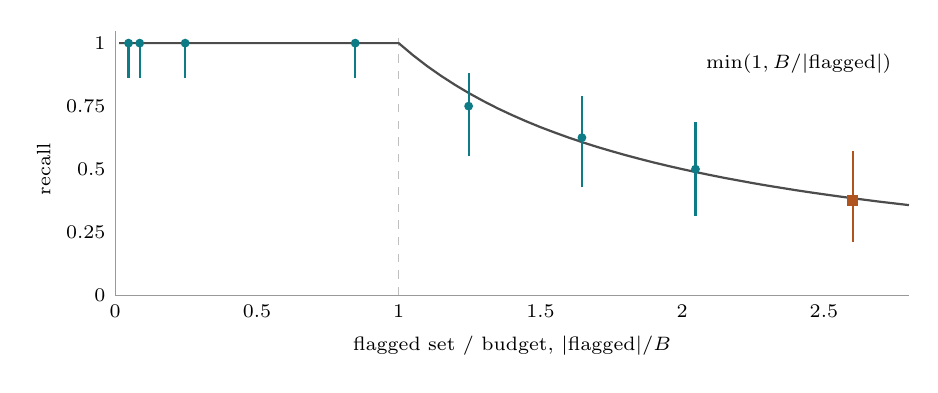
\begin{tikzpicture}[x=1cm,y=1cm]
  \draw[black!40] (0,0) -- (10.08,0);
  \draw[black!40] (0,0) -- (0,3.36);
  \foreach \y in {0,0.25,0.5,0.75,1}
    \node[anchor=east,font=\scriptsize] at (0,{\y*3.2}) {\y};
  \foreach \x in {0,0.5,1,1.5,2,2.5}
    \node[anchor=north,font=\scriptsize] at ({\x*3.6},0) {\x};
  \draw[black!25,dashed] (3.60,0) -- (3.60,3.36);
  \draw[black!70,thick] (0.05,3.200) -- (0.180,3.200) -- (0.360,3.200) -- (0.540,3.200) -- (0.720,3.200) -- (0.900,3.200) -- (1.080,3.200) -- (1.260,3.200) -- (1.440,3.200) -- (1.620,3.200) -- (1.800,3.200) -- (1.980,3.200) -- (2.160,3.200) -- (2.340,3.200) -- (2.520,3.200) -- (2.700,3.200) -- (2.880,3.200) -- (3.060,3.200) -- (3.240,3.200) -- (3.420,3.200) -- (3.600,3.200) -- (3.780,3.048) -- (3.960,2.909) -- (4.140,2.783) -- (4.320,2.667) -- (4.500,2.560) -- (4.680,2.462) -- (4.860,2.370) -- (5.040,2.286) -- (5.220,2.207) -- (5.400,2.133) -- (5.580,2.065) -- (5.760,2.000) -- (5.940,1.939) -- (6.120,1.882) -- (6.300,1.829) -- (6.480,1.778) -- (6.660,1.730) -- (6.840,1.684) -- (7.020,1.641) -- (7.200,1.600) -- (7.380,1.561) -- (7.560,1.524) -- (7.740,1.488) -- (7.920,1.455) -- (8.100,1.422) -- (8.280,1.391) -- (8.460,1.362) -- (8.640,1.333) -- (8.820,1.306) -- (9.000,1.280) -- (9.180,1.255) -- (9.360,1.231) -- (9.540,1.208) -- (9.720,1.185) -- (9.900,1.164) -- (10.080,1.143);
  \node[anchor=west,font=\scriptsize] at (7.38,2.94) {$\min(1, B/|\mathrm{flagged}|)$};
  \draw[tealaccent,thick] (0.169,2.758) -- (0.169,3.200);
  \fill[tealaccent] (0.169,3.200) circle (1.6pt);
  \draw[tealaccent,thick] (0.311,2.758) -- (0.311,3.200);
  \fill[tealaccent] (0.311,3.200) circle (1.6pt);
  \draw[tealaccent,thick] (0.888,2.758) -- (0.888,3.200);
  \fill[tealaccent] (0.888,3.200) circle (1.6pt);
  \draw[tealaccent,thick] (3.048,2.758) -- (3.048,3.200);
  \fill[tealaccent] (3.048,3.200) circle (1.6pt);
  \draw[tealaccent,thick] (4.488,1.763) -- (4.488,2.816);
  \fill[tealaccent] (4.488,2.400) circle (1.6pt);
  \draw[tealaccent,thick] (5.927,1.367) -- (5.927,2.523);
  \fill[tealaccent] (5.927,2.000) circle (1.6pt);
  \draw[tealaccent,thick] (7.369,1.006) -- (7.369,2.194);
  \fill[tealaccent] (7.369,1.600) circle (1.6pt);
  \draw[rustaccent,thick] (9.366,0.677) -- (9.366,1.833);
  \fill[rustaccent] (9.296,1.130) rectangle ++(0.14,0.14);
  \node[anchor=north,font=\scriptsize] at (5.04,-0.4) {flagged set / budget, $|\mathrm{flagged}|/B$};
  \node[anchor=south,rotate=90,font=\scriptsize] at (-0.7,1.60) {recall};
\end{tikzpicture}
\caption{\textbf{Precision is free until the budget binds.} Recall of the
coverage-1.00 oracle as false positives grow the flagged set (circles: synthetic
needles, $B{=}2048$, 24 queries each, 95\% Wilson intervals). The curve is
Eq.~\ref{eq:crowding}, not fitted. The square is real SQuAD QA at $B{=}512$,
where the flagged set is 1332 paragraph tokens; its uncompressed ceiling is
${\QACeiling}$, so the law predicts ${\CrowdPredScaled}$ to
${\CrowdPred}$ and ${\CrowdObs}$ is observed.}
\label{fig:crowding}
\end{figure}

\subsection{Stated}
\begin{quote}
A retention signal must identify \textbf{essentially every token} of an answer
span, and keep its \textbf{total flagged set within the budget}. It may be
entirely indiscriminate about which \emph{extra} tokens it keeps, so long as it
does not keep too many.
\end{quote}

\section{The specification as a test}\label{sec:test}

The coverage half can be measured \emph{without implementing a policy}: score
the stream, take the top $B$, and count the answer spans kept whole. Anything
well short of every span predicts end-to-end failure.

\paragraph{Validating it in both directions.} The degraded oracles are
candidates whose end-to-end recall is already measured across the whole
coverage range, so we screen them by replaying the flags their end-to-end runs
drew (Table~\ref{tab:coverage}, second column). The screen passes the
coverage-1.00 oracle, which succeeds on every query. It fails every degraded
oracle, keeping whole only the near-band spans that recency keeps anyway, and
none of them answers more than one middle-band query in seven. Spans kept whole
is a lower bound on recall rather than an estimate of it: at 0.75 coverage the
model still answers some queries whose span was damaged, mostly near the query,
where a damaged span sits beside intact context. The positive case is synthetic, since only an oracle
passes; we return to this in \S\ref{sec:limits}.

\paragraph{A prediction made in advance.} Surprisal, which scores each token by
$-\log p(\text{token}\mid\text{prefix})$ and so keeps what the context cannot
reconstruct, is a principled, free and non-positional candidate. On 16 spans
the screen rejected it locally at no cost, and \textbf{five predictions were
committed to version control before a GPU was rented.} All five held: needle
middle band $0/7$; needle near band $0/9$ against \texttt{recent}'s $10/14$;
needle overall $0/24$; QA overall $2/24$ with middle band $0/8$; and beating
\texttt{recent} on neither task. Every number landed at or below its predicted
bound.

\paragraph{Ten candidates.} Table~\ref{tab:screen} and Fig.~\ref{fig:screen}
screen every candidate on $\ScreenSpansNeedle$ needle spans and
$\ScreenSpansQA$ QA answer phrases. The first two rows were rejected end to
end before the screen existed. None passes: the best any signal does on either
task is $\ScreenBestWhole$ spans whole. On QA, spans kept whole must be read
against the random control's $\RandomWholeQA$: many answer phrases are one or
two tokens, and chance keeps a quarter of those.

\begin{table}[h]\centering\small
\TabScreen
\caption{Ten candidates, none passing. Coverage at $B{=}2048$; chance is $0.25$.}
\label{tab:screen}
\end{table}

\begin{figure}[t]
\centering
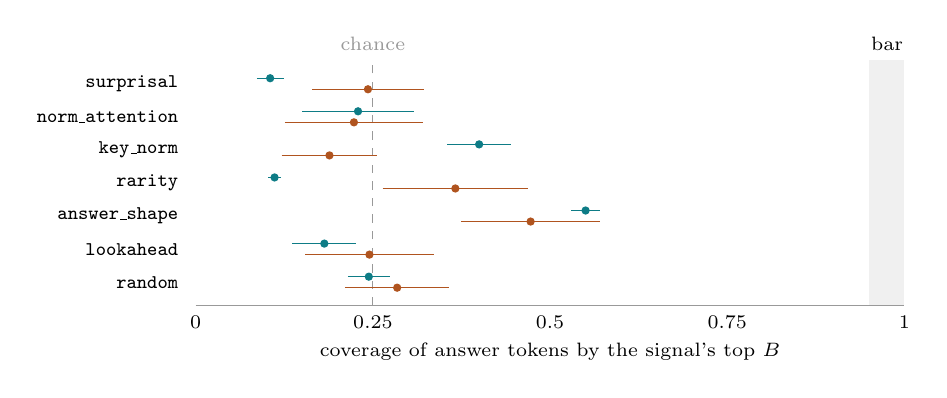
\begin{tikzpicture}[x=1cm,y=1cm]
  \fill[black!6] (8.55,-2.82) rectangle (9.00,0.3);
  \draw[black!40,dashed] (2.25,-2.82) -- (2.25,0.3)
    node[anchor=south,font=\scriptsize] {chance};
  \node[anchor=south,font=\scriptsize] at (8.78,0.3) {bar};
  \node[anchor=east,font=\scriptsize\ttfamily] at (-0.1,0.00) {surprisal};
  \draw[tealaccent] (0.775,0.07) -- (1.115,0.07);
  \fill[tealaccent] (0.945,0.07) circle (1.5pt);
  \draw[rustaccent] (1.479,-0.07) -- (2.895,-0.07);
  \fill[rustaccent] (2.187,-0.07) circle (1.5pt);
  \node[anchor=east,font=\scriptsize\ttfamily] at (-0.1,-0.42) {norm\_attention};
  \draw[tealaccent] (1.355,-0.35) -- (2.767,-0.35);
  \fill[tealaccent] (2.061,-0.35) circle (1.5pt);
  \draw[rustaccent] (1.133,-0.49) -- (2.886,-0.49);
  \fill[rustaccent] (2.009,-0.49) circle (1.5pt);
  \node[anchor=east,font=\scriptsize\ttfamily] at (-0.1,-0.84) {key\_norm};
  \draw[tealaccent] (3.193,-0.77) -- (4.004,-0.77);
  \fill[tealaccent] (3.599,-0.77) circle (1.5pt);
  \draw[rustaccent] (1.092,-0.91) -- (2.303,-0.91);
  \fill[rustaccent] (1.698,-0.91) circle (1.5pt);
  \node[anchor=east,font=\scriptsize\ttfamily] at (-0.1,-1.26) {rarity};
  \draw[tealaccent] (0.922,-1.19) -- (1.081,-1.19);
  \fill[tealaccent] (1.001,-1.19) circle (1.5pt);
  \draw[rustaccent] (2.373,-1.33) -- (4.222,-1.33);
  \fill[rustaccent] (3.297,-1.33) circle (1.5pt);
  \node[anchor=east,font=\scriptsize\ttfamily] at (-0.1,-1.68) {answer\_shape};
  \draw[tealaccent] (4.766,-1.61) -- (5.136,-1.61);
  \fill[tealaccent] (4.951,-1.61) circle (1.5pt);
  \draw[rustaccent] (3.375,-1.75) -- (5.131,-1.75);
  \fill[rustaccent] (4.253,-1.75) circle (1.5pt);
  \node[anchor=east,font=\scriptsize\ttfamily] at (-0.1,-2.10) {lookahead};
  \draw[tealaccent] (1.226,-2.03) -- (2.041,-2.03);
  \fill[tealaccent] (1.633,-2.03) circle (1.5pt);
  \draw[rustaccent] (1.391,-2.17) -- (3.021,-2.17);
  \fill[rustaccent] (2.206,-2.17) circle (1.5pt);
  \node[anchor=east,font=\scriptsize\ttfamily] at (-0.1,-2.52) {random};
  \draw[tealaccent] (1.933,-2.45) -- (2.462,-2.45);
  \fill[tealaccent] (2.198,-2.45) circle (1.5pt);
  \draw[rustaccent] (1.894,-2.59) -- (3.222,-2.59);
  \fill[rustaccent] (2.558,-2.59) circle (1.5pt);
  \draw[black!40] (0,-2.82) -- (9.00,-2.82);
  \foreach \x in {0,0.25,0.5,0.75,1}
    \node[anchor=north,font=\scriptsize] at ({\x*9.0},-2.82) {\x};
  \node[anchor=north,font=\scriptsize] at (4.50,-3.17)
    {coverage of answer tokens by the signal's top $B$};
\end{tikzpicture}
\caption{\textbf{No candidate approaches the bar.} Mean coverage over answer
spans at $B{=}2048$ with 95\% intervals, on synthetic needles
(\textcolor{tealaccent}{upper}) and real QA answer phrases
(\textcolor{rustaccent}{lower}); 64 and
62 spans. Chance is $B/L = 0.25$; the shaded band is where the specification
requires a signal to be.}
\label{fig:screen}
\end{figure}

Three entries carry the argument.

\textbf{\texttt{norm\_attention} fails, and it was the best available repair.}
Accumulated attention leans toward the start of the stream, because the sum
runs over a variable number of query rows and early tokens are visible to more
of them. Dividing by that count is the obvious fix. It lands near chance on
both tasks ($\NormattentionNeedle$ and $\NormattentionQA$). Removing the
positional bias does not uncover a utility signal underneath; it removes the
bias that produced H2O's only wins.

\textbf{\texttt{answer\_shape} is the strongest signal found and still fails.}
At $\AnswerShapeRatio\times$ chance on needles it does what it was built to do:
it flags digits, and the answers are digits. It is a prior written with
knowledge of the answer \emph{format}, and it keeps $\AnswerShapeWholeNeedle$
needle spans whole, because it ranks digits against every other digit-like
token in the stream and half a six-digit code is worth nothing. On QA it is
also the strongest signal, keeping $\AnswerShapeWholeQA$ answer phrases whole
against random's $\RandomWholeQA$: a real prior, and still three quarters
short of the bar. Knowing the form of the answer is not enough.

\textbf{\texttt{lookahead} fails, and it was the hardest test.} Every other
candidate must infer a token's future from its past. This one is \emph{given}
128 tokens of that future: the attention a token receives from the following
chunk, implementable by delaying compression by a single chunk. It scores
$\LookaheadNeedle$ on needles, below chance, and $\LookaheadQA$ on QA, at
chance. A chunk's attention to its predecessor
is dominated by local continuation, so short-range lookahead mostly measures
very local recency, which says nothing about being queried thousands of tokens
later.

\begin{quote}
The information that determines a token's retention value is not in its past,
and not in its immediate future either. It is in a query that has not arrived.
\end{quote}

\section{Why position-based rules cannot clear the bar}\label{sec:mech}

\begin{figure}[t]
\centering
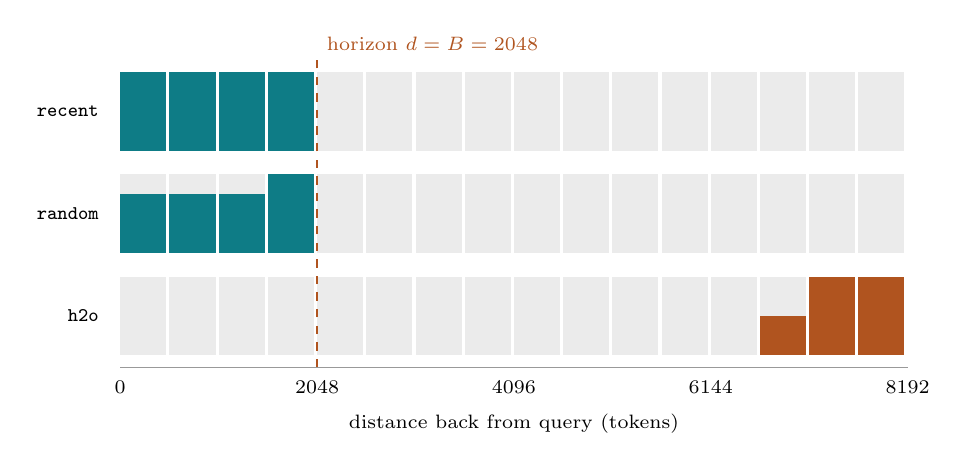
\begin{tikzpicture}[x=1cm,y=1cm]
% recent
    \fill[black!8] (0.000,2.60) rectangle ++(0.585,1.0);
    \fill[tealaccent] (0.000,2.60) rectangle ++(0.585,1.000);
    \fill[black!8] (0.625,2.60) rectangle ++(0.585,1.0);
    \fill[tealaccent] (0.625,2.60) rectangle ++(0.585,1.000);
    \fill[black!8] (1.250,2.60) rectangle ++(0.585,1.0);
    \fill[tealaccent] (1.250,2.60) rectangle ++(0.585,1.000);
    \fill[black!8] (1.875,2.60) rectangle ++(0.585,1.0);
    \fill[tealaccent] (1.875,2.60) rectangle ++(0.585,1.000);
    \fill[black!8] (2.500,2.60) rectangle ++(0.585,1.0);
    \fill[black!8] (3.125,2.60) rectangle ++(0.585,1.0);
    \fill[black!8] (3.750,2.60) rectangle ++(0.585,1.0);
    \fill[black!8] (4.375,2.60) rectangle ++(0.585,1.0);
    \fill[black!8] (5.000,2.60) rectangle ++(0.585,1.0);
    \fill[black!8] (5.625,2.60) rectangle ++(0.585,1.0);
    \fill[black!8] (6.250,2.60) rectangle ++(0.585,1.0);
    \fill[black!8] (6.875,2.60) rectangle ++(0.585,1.0);
    \fill[black!8] (7.500,2.60) rectangle ++(0.585,1.0);
    \fill[black!8] (8.125,2.60) rectangle ++(0.585,1.0);
    \fill[black!8] (8.750,2.60) rectangle ++(0.585,1.0);
    \fill[black!8] (9.375,2.60) rectangle ++(0.585,1.0);
  \node[anchor=east,font=\scriptsize\ttfamily] at (-0.15,3.1) {recent};
% random
    \fill[black!8] (0.000,1.30) rectangle ++(0.585,1.0);
    \fill[tealaccent] (0.000,1.30) rectangle ++(0.585,0.750);
    \fill[black!8] (0.625,1.30) rectangle ++(0.585,1.0);
    \fill[tealaccent] (0.625,1.30) rectangle ++(0.585,0.750);
    \fill[black!8] (1.250,1.30) rectangle ++(0.585,1.0);
    \fill[tealaccent] (1.250,1.30) rectangle ++(0.585,0.750);
    \fill[black!8] (1.875,1.30) rectangle ++(0.585,1.0);
    \fill[tealaccent] (1.875,1.30) rectangle ++(0.585,1.000);
    \fill[black!8] (2.500,1.30) rectangle ++(0.585,1.0);
    \fill[black!8] (3.125,1.30) rectangle ++(0.585,1.0);
    \fill[black!8] (3.750,1.30) rectangle ++(0.585,1.0);
    \fill[black!8] (4.375,1.30) rectangle ++(0.585,1.0);
    \fill[black!8] (5.000,1.30) rectangle ++(0.585,1.0);
    \fill[black!8] (5.625,1.30) rectangle ++(0.585,1.0);
    \fill[black!8] (6.250,1.30) rectangle ++(0.585,1.0);
    \fill[black!8] (6.875,1.30) rectangle ++(0.585,1.0);
    \fill[black!8] (7.500,1.30) rectangle ++(0.585,1.0);
    \fill[black!8] (8.125,1.30) rectangle ++(0.585,1.0);
    \fill[black!8] (8.750,1.30) rectangle ++(0.585,1.0);
    \fill[black!8] (9.375,1.30) rectangle ++(0.585,1.0);
  \node[anchor=east,font=\scriptsize\ttfamily] at (-0.15,1.8) {random};
% h2o
    \fill[black!8] (0.000,0.00) rectangle ++(0.585,1.0);
    \fill[black!8] (0.625,0.00) rectangle ++(0.585,1.0);
    \fill[black!8] (1.250,0.00) rectangle ++(0.585,1.0);
    \fill[black!8] (1.875,0.00) rectangle ++(0.585,1.0);
    \fill[black!8] (2.500,0.00) rectangle ++(0.585,1.0);
    \fill[black!8] (3.125,0.00) rectangle ++(0.585,1.0);
    \fill[black!8] (3.750,0.00) rectangle ++(0.585,1.0);
    \fill[black!8] (4.375,0.00) rectangle ++(0.585,1.0);
    \fill[black!8] (5.000,0.00) rectangle ++(0.585,1.0);
    \fill[black!8] (5.625,0.00) rectangle ++(0.585,1.0);
    \fill[black!8] (6.250,0.00) rectangle ++(0.585,1.0);
    \fill[black!8] (6.875,0.00) rectangle ++(0.585,1.0);
    \fill[black!8] (7.500,0.00) rectangle ++(0.585,1.0);
    \fill[black!8] (8.125,0.00) rectangle ++(0.585,1.0);
    \fill[rustaccent] (8.125,0.00) rectangle ++(0.585,0.500);
    \fill[black!8] (8.750,0.00) rectangle ++(0.585,1.0);
    \fill[rustaccent] (8.750,0.00) rectangle ++(0.585,1.000);
    \fill[black!8] (9.375,0.00) rectangle ++(0.585,1.0);
    \fill[rustaccent] (9.375,0.00) rectangle ++(0.585,1.000);
  \node[anchor=east,font=\scriptsize\ttfamily] at (-0.15,0.5) {h2o};
% horizon
  \draw[rustaccent,dashed,thick] (2.500,-0.15) -- (2.500,3.75);
  \node[anchor=south west,font=\scriptsize,rustaccent] at (2.500,3.75)
    {horizon $d=B=2048$};
% axis
  \draw[black!40] (0,-0.15) -- (10,-0.15);
  \foreach \f/\l in {0/0, 0.25/2048, 0.5/4096, 0.75/6144, 1.0/8192}
    \node[anchor=north,font=\scriptsize] at ({\f*10},-0.2) {\l};
  \node[anchor=north,font=\scriptsize] at (5,-0.62)
    {distance back from query (tokens)};
\end{tikzpicture}
\caption{\textbf{The retention horizon.} Recall in 512-token distance bins at
$B{=}2048$ (Qwen3-1.7B, 4 seeds $\times$ 16 needles); bar height is recall,
grey is the empty cell. \texttt{recent} holds $1.00$ out to $d{=}B$ and
scores nothing beyond it; \texttt{h2o} is the mirror image anchored to
the start of the stream. Neither reaches the ${\approx}4000$ tokens between
them.}
\label{fig:horizon}
\end{figure}

Under admission at rate $p$ followed by FIFO eviction to budget $B$, occupancy
saturates and the cache becomes a contiguous window over the most recent $B/p$
raw positions:
\begin{equation}
  P(\text{token resident at distance } d) =
  \begin{cases} p & d < B/p \\ 0 & \text{otherwise.}\end{cases}
  \label{eq:horizon}
\end{equation}
For \texttt{recent} ($p{=}1$), every needle inside $d{=}B$ is answered and
$\RecentBeyond$ beyond it (95\% upper bound $\RecentBeyondUpper$). At
$p{=}0.5$ the horizon should move to 4096; we observe $\HorizonInside$ inside
and $\HorizonBeyond$ beyond (upper bound $\HorizonBeyondUpper$).
Eq.~\ref{eq:horizon} governs \emph{token} residency, and recall needs every
token of an $L_a$-token answer, so the in-horizon plateau is roughly
$p^{L_a}$ rather than $p$. That is why the plateau is low. What the test
confirms is the horizon.

Beyond the horizon, the mechanism gives survival probability zero, not merely
a small one: any rule that does not actively protect a token past $B/p$ loses
it. Recency is therefore not a design choice but the behaviour every
uninformed rule decays onto. \texttt{h2o} shows the mirror image
(Fig.~\ref{fig:horizon}). At $B{=}2048$, \texttt{recent} answers $10/14$ near
and $0/14$ far; \texttt{h2o} answers $0/14$ near and $8/14$ far. Both are
functions of position, neither of utility, and neither reaches the middle.

\paragraph{The horizon depends on tokens stored, not bytes.} Eq.~\ref{eq:horizon}
is stated in tokens, so anything that fits more tokens into the same memory
should move the horizon and nothing else. We test this by quantising the cache
rather than changing the policy: with the budget fixed in bits and FIFO
unchanged, int2 storage (keys quantised per channel, as in
\citealp{liu2024kivi}) holds \GradedIntTwoLargeTokens tokens where fp16 holds
\GradedFpLargeTokens. Recall rises from \GradedFpLarge to
\GradedIntTwoLarge $\GradedIntTwoLargeCI$, and the middle band from
\GradedFpLargeMid to \GradedIntTwoLargeMid: the same FIFO rule, the same
memory, the horizon moved past the middle of the context. Two rungs below int2
(int1, and averaging adjacent entries) keep still more tokens and answer
nothing, so fidelity per token is a floor, not a free parameter. A ladder that
spends bits by priority --- keeping high-scoring chunks at fp16 and stepping the
rest down under a KL test against the incoming text --- loses to uniform int2
at every budget (\GradedKlLarge against \GradedIntTwoLarge), because it buys
precision with the tokens the horizon needs.

\section{A signal that passes the test}\label{sec:probe}

A screen that rejects every candidate cannot be distinguished from a screen
that rejects everything. This section supplies the missing case: a signal that
is realisable, passes the screen, and then reaches the oracle's recall. It also
shows how narrow the resulting method is.

\paragraph{The signal.} Logistic regression on the frozen model's layer-14
hidden state, one score per token, fitted on six streams whose answer spans are
labelled and tested on streams it never saw. The feature is the hidden state a
causal forward pass has already computed at the moment the token is written, so
the signal is write-time in the sense \S\ref{sec:setup} requires; the labels
are supervision, used only in fitting. This is not a solution to the problem
the paper poses --- the labels presuppose knowing what the answers look like ---
but it is a realisable scoring rule, and the screen does not know how it was
obtained.

\begin{table}[h]\centering\small
\TabProbe
\caption{The probe against the screen's two predictions. In-task on needles it
passes the screen and matches the oracle; on QA it fails the screen and then
fails end to end, at \texttt{recent}'s level.}
\label{tab:probe}
\end{table}

\paragraph{Both predictions hold.} On needles the probe keeps
$\ProbeNeedleNeedle$ $\ProbeNeedleNeedleCI$ spans whole against the random
control's $\ProbeNeedleNeedleRand$ --- the first realisable signal here to pass
the screen --- and end to end it answers \ProbeESmall
$\ProbeESmallCI$ at $B{=}1024$ and \ProbeELarge at $B{=}2048$, with the
middle band at \ProbeESmallMid, against \texttt{recent}'s \RecentESmall and
\RecentESmallMid. That is the oracle's ceiling (Table~\ref{tab:oracle})
reached by a signal that reads only what the model computed at write time. On
QA the same recipe keeps $\ProbeQaQa$ $\ProbeQaQaCI$ spans whole against
random's $\ProbeQaQaRand$: above chance, far short of the bar, so the screen
predicts failure. It fails, answering \ProbeEQASmall and \ProbeEQALarge,
neither better than \texttt{recent}'s \RecentEQASmall and \RecentEQALarge.
The screen now has a confirmed prediction in each direction from one realisable
signal class, which is what \S\ref{sec:limits} of the earlier draft asked for.

\paragraph{What it transfers across, and what it does not.} Two shifts leave it
working. Fitted on needles whose answers are six-digit codes and tested on
needles whose answers are phrases, it answers \ProbeEStyleSmall
$\ProbeEStyleSmallCI$ against \texttt{recent}'s \RecentEStyleSmall, with the
middle band at \ProbeEStyleSmallMid --- below its in-distribution
\ProbeESmall, still far above recency. Refitted and rerun on a second model,
SmolLM2-1.7B, it answers \ProbeESmolSmall $\ProbeESmolSmallCI$ against
\RecentESmolSmall, so the recipe is not a quirk of one model's activations.
The boundary it does not cross is the task: fitted on QA it ranks needle tokens
no better than chance ($\ProbeQaNeedle$ spans whole, random
$\ProbeQaNeedleRand$), and fitted on needles it keeps $\ProbeNeedleQa$ QA
answer phrases whole. What the probe learns survives a change of surface form
and of backbone, and does not survive a change of what counts as an answer.

\paragraph{What this changes.} The capacity the oracle demonstrates is
reachable, cheaply, when the task distribution is known in advance: a linear
read of existing activations is enough. What remains unsolved is the
task-agnostic case, which is the case a general compression method faces. The
paper's negative result should therefore be read as scoped: no \emph{task-%
agnostic} write-time signal we tested clears the bar, and the one signal that
clears it does so by being told, in training, what this task's answers look
like. Finally, the two gains do not compose: pairing the probe with int2
storage costs recall (\ProbeIntTwoESmall against \ProbeESmall), because
extra reach is worthless once the right tokens are already being kept.

\section{A constraint the specification misses}\label{sec:frag}

The specification concerns \emph{which} tokens are retained, not how they are
arranged, and arrangement matters. We hold the stream, needles, distances,
flagged-token count (1600) and recency fill constant, and vary only the number
of contiguous runs the retained evidence occupies.

\begin{table}[h]\centering\small
\TabFrag
\caption{Recall against the number of contiguous runs holding the same 1600
retained tokens, 24 queries per cell.}
\label{tab:frag}
\end{table}

Fisher's exact test, 8 runs against 4 on SmolLM2: $p = \FragP$
(Table~\ref{tab:frag}). The near band is perfect at every setting, so the loss
is in the middle and far bands, and width does not explain it: a separate
sweep varied width at fixed count over a $13\times$ range and moved recall only
from $0.50$ to $0.58$. Qwen3-1.7B is barely affected, so this is a
model-dependent sensitivity. That fragmentation harms compressed caches is
known \citep{yang2026ams}; what this adds is the controlled attribution to
fragment \emph{count}, and a consequence for \S\ref{sec:spec}: a signal can
meet the specification exactly and still fail by delivering the right tokens
in too many pieces.

\section{Limitations}\label{sec:limits}

\textbf{The signal that passes the screen is supervised and task-specific}
(\S\ref{sec:probe}). It is fitted on labelled answer spans from the task it is
then tested on, and it does not survive a change of task or of answer form. It
establishes that the screen is not uselessly conservative and that the oracle's
capacity is reachable; it does not supply a task-agnostic signal, which is what
a general compression method needs.
\textbf{The oracle is an upper bound, not a method}: it requires knowing the
answers in advance. This paper specifies a target, supplies a test, and shows
the target is reachable under supervision.
\textbf{The probe's generalisation is measured coarsely}: one answer-form shift
and one second model, at one budget, with 24 queries each.
\textbf{Small samples.} Most cells hold 24--64 queries or spans; every
proportion is reported with its interval.
\textbf{Short contexts and two task families.} Streams are 8192 tokens, both
tasks have short answers, and neither is a published benchmark such as RULER
\citep{hsieh2024ruler}. The real-QA task discriminates only on Qwen3-1.7B.
\textbf{Three models, 1.7B--8B}, two from one family.
\textbf{Scoring rules, not systems} (\S\ref{sec:setup}).
\textbf{One eviction regime}: FIFO eviction, a fixed per-layer budget, and
decisions shared across layers (the last forced by a single global attention
mask).
\textbf{The plateau of Eq.~\ref{eq:horizon} has no clean quantitative model};
it falls roughly as $p^{L_a}$, with an effective $L_a$ that varies.
\textbf{The coverage curve is measured on the synthetic task only}; its
transfer to QA rests on Eq.~\ref{eq:crowding}, which was checked there, not on
a second coverage sweep.

\section{Related work}\label{sec:related}

\textbf{Position bias without compression.} \citet{liu2024lost} show a U-shaped
accuracy curve over the position of relevant information in \emph{uncompressed}
context. Our uncompressed baseline answers every needle in every band on all
three models, so at these lengths the middle is answered perfectly without a
budget: the effect we start from is created by compression, not inherited from
the model.

\textbf{Evaluating compression.} Benchmarks compare compression methods across
tasks \citep{yuan2024kvbench} and across the life cycle of a shared cache
\citep{li2025scbench}; RULER \citep{hsieh2024ruler} measures effective context
length with synthetic retrieval tasks. \citet{indexmem2026} report
needle-in-a-haystack heatmaps over context length and depth and observe
position-dependent failure of SnapKV and PyramidKV. Reporting recall by
position is therefore not new; \S\ref{sec:mech} adds the horizon mechanism and
the complementarity of the two rule families.

\textbf{Fragmentation.} \citet{yang2026ams} name \emph{region wipe-out}, where
global top-$k$ selection evicts contiguous blocks, and propose region-aware
segment quotas. \S\ref{sec:frag}'s phenomenon and its remedy are theirs, in a
decoding-time reasoning setting; our contribution there is the controlled
attribution to fragment count.

\textbf{Non-uniform damage.} \citet{chen2025pitfalls} find that under
multi-instruction prompting some instructions degrade far faster than others.
The theme is the same on a different axis: their unit is an instruction, ours a
fact at a distance.

\textbf{Quantised caches.} KIVI \citep{liu2024kivi} stores keys per channel and
values per token at 2 bits with no tuning. Our use of it is diagnostic rather
than a contribution: quantisation changes how many tokens a budget holds, which
is the one free variable in Eq.~\ref{eq:horizon}, so it is the cleanest way to
move the horizon without touching the policy (\S\ref{sec:mech}).

\textbf{Learned and query-aware retention.} Write-time admission with a frozen
backbone \citep{kvadmission2025}; reinforcement learning for eviction, trained
on a reward derived from future utility \citep{learningtoevict2026}; learned
routing for KV allocation \citep{triroute2026}. Query-aware methods such as
Quest \citep{tang2024quest} select cache pages using the current query at
decode time, which sidesteps the problem studied here by keeping the full
cache resident.

\textbf{What is new} is not that compression hurts, nor where. It is the
\emph{target}---an oracle establishing that the capacity exists, and two laws
saying what a signal must achieve to reach it---and the \emph{test} that turns
the target into a rejection criterion costing nothing to apply.

\textbf{What we do not claim.} We did not run H2O, SnapKV or StreamingLLM as
published systems and do not report that they fail on their own benchmarks.
Whether the full systems inherit these effects is our prediction, not our
measurement.

\section*{Reproducibility}

Every experiment uses frozen public checkpoints and fixed seeds. The screen
(\S\ref{sec:test}) and the degraded-oracle replay run on a laptop (Apple M4);
end-to-end runs used a single rented RTX 3090. Every number in this
paper is generated from per-query result files by one script, so the text
cannot drift from the data. The harness is covered by unit tests, including a
bit-identity test against the stock cache.

\section*{Code availability}

Code, per-query results and the script that generates every table and figure
are available at
\begin{center}\url{https://github.com/SrujanPendurthi/kvAdmission}\end{center}

\bibliographystyle{plainnat}
\bibliography{refs}
\end{document}
